\chapter{Ricevitore numerico}

\begin{figure}[h]
    \centering
    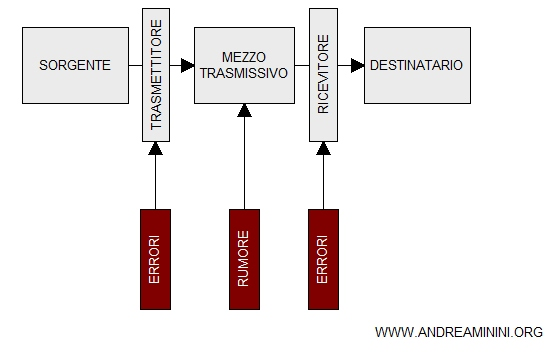
\includegraphics[scale = 0.8]{schema-sistema-telecomunicazioni.jpg}
\end{figure}

\newpage 

\section{Ricevitore ottimo}
\footnote{Slide del prof | Ricevitore numerico | pag 1 \\  
Appunti di Damiano | pag 1 \\
Slide | Ricevitore numerico | pag 1 \\
Appunti | 2025-04-01 | pag 5 - 6
}

Consideriamo questo modello per la trasmissione di un segnale ricevuto da un ricevitore: 

\begin{figure}[h]
    \centering
    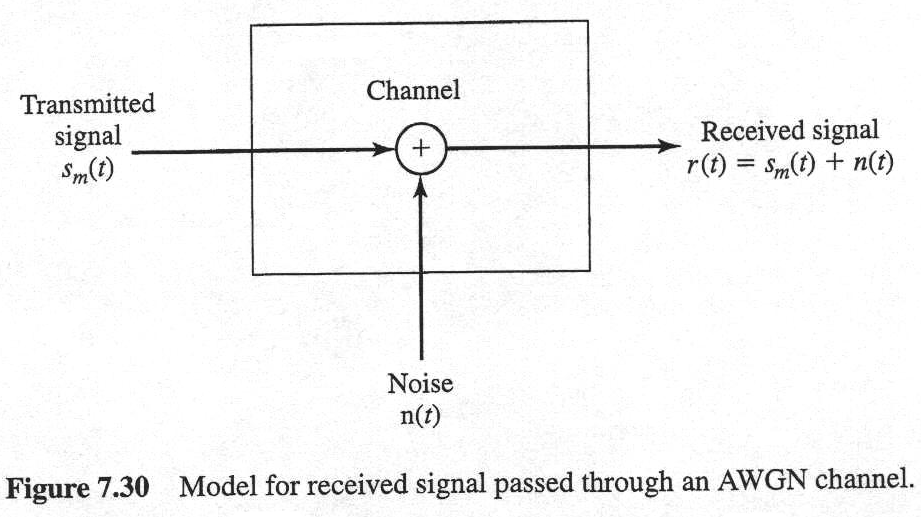
\includegraphics[scale = 0.8]{Ricevitore numerico.png}
\end{figure}

Questo tipo di modello vale sotto queste ipotesi: 

\begin{itemize}
    \item Non si considera l'attenuazione nel canale, quindi il segnale trasmesso $s_m (t)$ a sinistra della figura è lo stesso di quello a destra
    \item il rumore n(t) è AWGN (Additive White Gaussian Noise), quindi è solo additivo, e non si considerano altri tipi di rumore
\end{itemize}

Essendo il rumore n(t) AWGN, nello spettro il rumore sarà additivo e costante in frequenza: 

\begin{figure}[h]
    \centering
    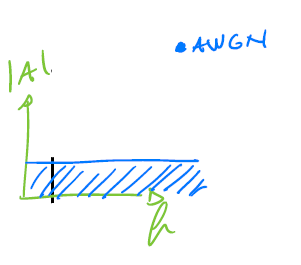
\includegraphics[scale = 1]{Spettro in frequenza del rumore AWGN.PNG}
\end{figure}

Dato questo modello, l'obbiettivo è progettare un ricevitore che sia ottimo, 
nel senso che minimizzi la probabilità di errore. \newline 

\begin{tcolorbox}
    Rimarchiamo una caratteristica rispetto al caso analogico. \newline 

    Siccome adesso abbiamo a che fare con sistemi numerici, 
    il rumore impatta la probabilità di errore del simbolo, 
    non il segnale analogico tutto perchè, nei ricevitori numerici, 
    i simboli fanno parte di un alfabeto discreto, e non infinito come nelle modulazioni analogiche. 
\end{tcolorbox}

Per i nostri obbiettivi, è meglio suddividere il ricevitore in due parti (partendo dal segnale ricevuto $r(t)$): 

\begin{itemize}
    \item Demodulatore del segnale ricevuto 
    \item Decisore
\end{itemize}

Il compito del demodulatore è quello di convertire la forma d'onda ricevuta r(t) in un vettore N-dimensione $\overrightarrow{r}$ con le seguenti componenti: 

{
    \Large 
    \begin{equation}
        \overrightarrow{r} = (r_1, r_2, \dots, r_N)
    \end{equation}
}

Il vettore $\overrightarrow{r}$ è la rappresentazione geometrica nella N-dimensione in cui i segnali, cioè simboli, 
dell'alfabeto di trasmissione. \newline 

Nel caso ideale in cui il rumore n(t) è nullo: 

{
    \Large 
    \begin{equation}
        \overrightarrow{r} = \overrightarrow{s_m}
    \end{equation}
}

cioè, il simbolo ricevuto $\overrightarrow{r}$ è uguale a il simbolo trasmesso $\overrightarrow{s_m}$. \newline 

Ma, siccome il rumore n(t) non è nullo e inciderà sul segnale trasmesso $s_m (t)$, 
allora sarà il compito del decisore decidere, dall'osservazione di $\overrightarrow{r}$, 
quale degli M simboli possibili è stato trasmesso facendo una stima, perchè il rumore è un processo stocastico, cioè probabilistico. \newline 

Dalla stima del simbolo trasmesso, 
è poi possibile recuperare l'informazione originale. \newline 

\newpage 

\section{Demodulatore (ricevitore) a correlatore}
\footnote{Slide del prof | Ricevitore numerico | pag 2 \\  
Appunti di Damiano | pag 2 \\
Slide | Ricevitore numerico | pag 2 \\
Appunti | 2025-04-01 | pag 6 \\
Appunti | 2025-04-04 | pag 2 - 3
}

Di seguito lo schema del demodulatore (ricevitore) a correlatore (con le note): 

\begin{figure}[h]
    \centering
    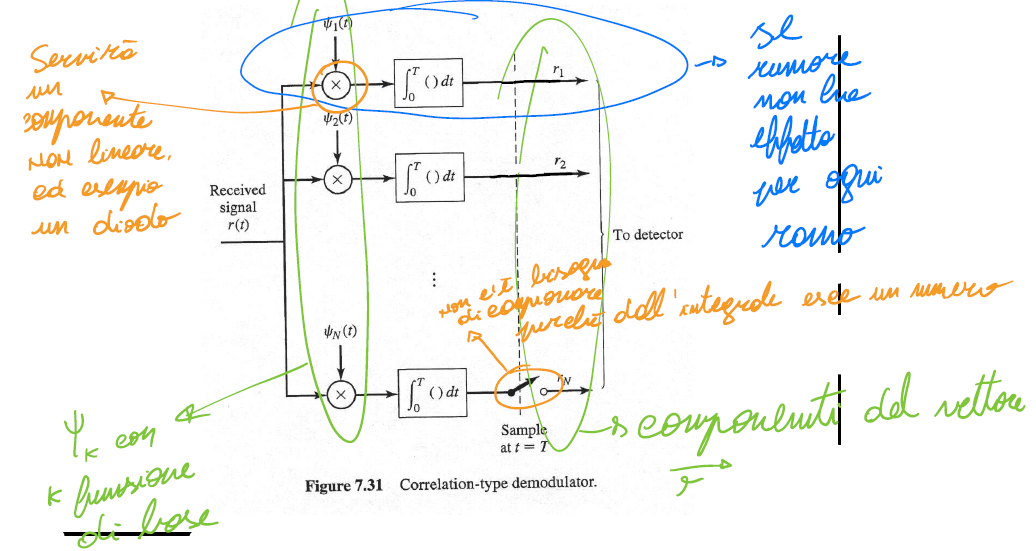
\includegraphics[scale = 0.8]{Demodulatore (ricevitore) a correlatore schema con note.PNG}
\end{figure}

Alcune note che non ho evidenziato nello schema: 

\begin{itemize}
    \item Il blocco integratore di ogni ramo è visto, in frequenza, come un filtro passa-basso 
    \item $\Psi_k (t)$ è un versore della base N-dimensione 
\end{itemize}

Sapendo che quello che riceviamo dal demodulatore è il vettore $\overrightarrow{r}$: 

{
    \Large 
    \begin{equation}
        \overrightarrow{r} = \overrightarrow{s_m} + \overrightarrow{n}
    \end{equation}
}

cioè il vettore ricevuto $\overrightarrow{r}$ è la somma del segnale trasmesso $\overrightarrow{s_m} $ e il vettore rumore $\overrightarrow{n}$. \newline 

Possiamo scomporre i vettori nei loro componenti. \newline 

Se consideriamo k: 

{
    \Large 
    \begin{equation}
        k = 1, 2, \dots, N
    \end{equation}
}

dove N è la dimensione dello spazio, 
possiamo considerare ogni ramo del demodulatore un singolo componente del vettore $\overrightarrow{r}$, 
quindi anche di $\overrightarrow{s_m}$ e di $\overrightarrow{r}$. \newline 

Se consideriamo il singolo ramo del demodulatore,  
possiamo esprimere matematicamente il segnale ricevuto come: 

{
    \Large 
    \begin{equation}
        \begin{split}
        \int_{0}^{T}
        r(t) \cdot \Psi_k (t) 
        dt 
        &=
        \int_{0}^{T}
        \left[
            s_m (t) + n(t)
        \right]
        \cdot 
        \Psi_k (t)
        dt
        \\
        &=
        \int_{0}^{T}
        s_m (t)
        \cdot 
        \Psi_k (t)
        dt
        + 
        \int_{0}^{T}
        n(t)
        \cdot 
        \Psi_k (t)
        dt
        \end{split}
    \end{equation}
}

Sapendo che il singolo elemento del vettore del segnale ricevuto $\overrightarrow{r}$ è composto da: 

{
    \Large
    \begin{equation}
        r_k = s_{mk} + n_k \text{ per } k = 1, 2, \dots, N
    \end{equation}
}

allora possiamo scrivere la equazione precedente nei vari componenti. \newline 

Per quanto riguarda il segnale trasmesso: 

{
    \Large 
    \begin{equation}
        \begin{split}
        \int_{0}^{T}
        s_m (t)
        &\cdot 
        \Psi_k (t)
        dt
        \\
        &\downarrow
        \\
        s_{mk} 
        =
        \int_{0}^{T}
        s_m (t)
        &\cdot 
        \Psi_k (t)
        dt 
        \text{ per } k = 1, 2, \dots, N
        \end{split}
    \end{equation}
}

Per quanto riguarda il rumore: 

{
    \Large 
    \begin{equation}
        \begin{split}
        \int_{0}^{T}
        n(t)
        &\cdot 
        \Psi_k (t)
        dt
        \\
        &\downarrow
        \\
        n_{k} 
        =
        \int_{0}^{T}
        n (t)
        &\cdot 
        \Psi_k (t)
        dt 
        \text{ per } k = 1, 2, \dots, N
        \end{split}
    \end{equation}
}

Considerando il segnale trasmesso s deterministico (anche se in realtà non lo è, ma per i nostri scopi lo è),
il rumore n è aleatorio perchè è un rumore termico: ciò comporta dell'errore sul singolo elemento della base $\Psi_k (t)$. \newline 

\newpage 

\subsection{Caratteristiche del rumore additivo}
\footnote{Slide del prof | Ricevitore numerico | pag 3 \\  
Appunti di Damiano | pag 3 \\
Slide | Ricevitore numerico | pag 3 \\
Appunti | 2025-04-04 | pag 2 - 3 \\
Appunti | 2025-07-21 Ricevimento | pag 5.3
}

\begin{tcolorbox}
    Un ripasso da Teoria dei Segnali per quanto riguarda il rumore additivo AWGN ed i calcoli che andremo a svolgere. \newline 

    Non dobbiamo sapere tutti i calcoli matematici qui riportati, però dobbiamo giustificare perchè traiamo queste conclusioni alla fine. \newline 

    Ripassa o tieni sotto, mentre leggi questo capitolo: \newline 

    \url{https://github.com/ciccio25/appunti-teoria-dei-segnali/blob/main/Appunti%20Teoria%20dei%20segnali.pdf} \\
    Capitolo 13 - Processi stocastici - pag 151 - 158
\end{tcolorbox}

Ritorniamo alla formula del rumore nel singolo ramo del demodulatore a correlatore: 

{
    \Large 
    \begin{equation}
        n_{k} 
        =
        \int_{0}^{T}
        n (t)
        \cdot 
        \Psi_k (t)
        dt 
        \text{ per } k = 1, 2, \dots, N
    \end{equation}
}

Per le considerazioni svolte nel precedente corso di Teoria dei Segnali, 
formalmente non possiamo indicare il rumore come un processo deterministico, 
bensì come processo probabilistico perchè il rumore è un fenomeno stocastico. \newline 

\begin{tcolorbox}
    Il rumore non è un fenomeno stoccafisso, si dice stocastico. \newline 

    Lo stoccafisso lo mangi dopo, adesso pensa allo studio
\end{tcolorbox}

Sapendo le caratteristiche del rumore AWGN, 
il rumore nel singolo ramo $n_k$ è una variabile gaussiana. \newline 

\begin{tcolorbox}
    Ripassa o tieni sotto, mentre leggi questo capitolo: \newline 

    \url{https://github.com/ciccio25/appunti-teoria-dei-segnali/blob/main/Appunti%20Teoria%20dei%20segnali.pdf} \\
    Capitolo 14 - Rumore termico - pag 161 - 163
\end{tcolorbox}

Se si è scelti un intervallo di tempo appropriato in base al disturbo, 
cioè si è scelti un un $[0, T]$ adeguato al disturbo, sappiamo che la media del rumore AWGN in un periodo vale: 

{
    \Large 
    \begin{equation}
        \mathbb{E} [n(t)]  = 0
    \end{equation}
}

dove con $\mathbb{E}$ si intende il valore medio del rumore n(t) nel periodo T. \newline 

Inoltre, considerando la formula di $n_k$: 

{
    \Large 
    \begin{equation}
        n_{k} 
        =
        \int_{0}^{T}
        n (t)
        \cdot 
        \Psi_k (t)
        dt 
        \text{ per } k = 1, 2, \dots, N
    \end{equation}
}

possiamo visualizzare l'integrale $\int_{0}^{T}$ una somma di tempi infinitesimi dt. \newline 

\begin{tcolorbox}
    Un altro minuto di silenzio per aver ucciso un altro matematico. \newline
    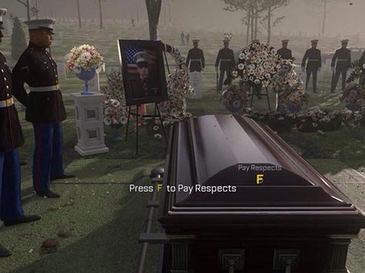
\includegraphics[scale = 0.8]{PressFtoPayRespects.jpg}
\end{tcolorbox}

Quindi, calcolando la media di $n_k$ nel periodo T vale, 
per qualsiasi valore di $\Psi_k (t)$: 

{
    \Large 
    \begin{equation}
        \begin{split}
        \mathbb{E} [n_k]
        &= 
        \int_{0}^{T}
        \mathbb{E} [n(t)] \cdot \Psi_k (t) dt 
        \\
        &= 
        \int_{0}^{T}
        0 \cdot \Psi_k (t) dt 
        \\
        &= 
        0
        \end{split}
    \end{equation}
}

Invece, se si vuole calcolare il valore medio tra due rami, cioè calcolare la loro correlazione, 
i calcoli diventano un pochino più complicati. \newline 

Considerando il rumore di due rami, cioè n e k, 
calcoliamo la correlazione tra i due rami: 

{
    \Large 
    \begin{equation}
        \mathbb{E} [n_k \cdot n_m]
        = 
        \int_{0}^{T}
        \int_{0}^{T}
        \mathbb{E} 
        \left[
            n(t) \cdot n(t + \tau)
        \right]
        \cdot 
        \Psi_k (t)
        \cdot 
        \Psi_m (t + \tau)
        dt 
        d\tau
    \end{equation}
}

Dalle proprietà del rumore termico, possiamo scrivere: 

{
    \Large 
    \begin{equation}
        \mathbb{E} 
        \left[
            n(t) \cdot n(t + \tau)
        \right]
        = 
        \mathbb{R} (\tau)
    \end{equation}
}

dove con $\mathbb{R} (\tau)$ si indica l'auto-correlazione del rumore termico. \newline 

Quindi, la correlazione diventa: 

{
    \Large 
    \begin{equation}
        \begin{split}
        \mathbb{E} [n_k \cdot n_m]
        &= 
        \int_{0}^{T}
        \int_{0}^{T}
        \mathbb{E} 
        \left[
            n(t) \cdot n(t + \tau)
        \right]
        \cdot 
        \Psi_k (t)
        \cdot 
        \Psi_m (t + \tau)
        dt 
        d\tau
        \\
        &\downarrow
        \\
        \mathbb{E} [n_k \cdot n_m]
        &= 
        \int_{0}^{T}
        \int_{0}^{T} 
       \mathbb{R} (\tau)
        \cdot 
        \Psi_k (t)
        \cdot 
        \Psi_m (t + \tau)
        dt 
        d\tau
        \end{split}
    \end{equation}
}

Sempre dal corso di Teoria segnali, sappiamo che: 

{
    \Large
    \begin{equation}
       \mathbb{R} (\tau)
       = 
       \frac{N_0}{2} \delta(\tau)
    \end{equation}
}

dove con $N_0$ si intende la densità spettrale del rumore. \newline 

Quindi:

{
    \Large 
    \begin{equation}
        \begin{split}
       \mathbb{E} [n_k \cdot n_m]
        &= 
        \int_{0}^{T}
        \int_{0}^{T} 
       \mathbb{R} (\tau)
        \cdot 
        \Psi_k (t)
        \cdot 
        \Psi_m (t + \tau)
        dt 
        d\tau
        \\
        &\downarrow
        \\
        \mathbb{E} [n_k \cdot n_m]
        &= 
        \int_{0}^{T}
        \int_{0}^{T} 
        \left[
        \frac{N_0}{2}
        \cdot 
        \delta (\tau)
        \right]
        \cdot 
        \Psi_k (t)
        \cdot 
        \Psi_m (t + \tau)
        dt 
        d\tau
        \end{split}
    \end{equation}
}

Andando a fare delle semplici sostituzioni algebriche: 

{
    \Large
    \begin{equation}
        \begin{split}
        \mathbb{E} [n_k \cdot n_m]
        &= 
        \int_{0}^{T}
        \int_{0}^{T} 
        \left[
        \frac{N_0}{2}
        \cdot 
        \delta (\tau)
        \right]
        \cdot 
        \Psi_k (t)
        \cdot 
        \Psi_m (t + \tau)
        dt 
        d\tau
        \\
        &= 
        \int_{0}^{T}
        \frac{N_0}{2}        
        \cdot
        \left[
        \int_{0}^{T}  
        \delta (\tau)
        \cdot 
        \Psi_m (t + \tau)
        d\tau
        \right]
        \cdot 
        \Psi_k (t)
        dt 
        \\
        &= 
        \int_{0}^{T}
        \frac{N_0}{2}        
        \cdot
        \Psi_m (t)
        \cdot 
        \Psi_k (t)
        dt 
        \\
        &=
        \frac{N_0}{2}        
        \cdot
        \int_{0}^{T}
        \Psi_m (t)
        \cdot 
        \Psi_k (t)
        dt 
        \\
        &= 
        \frac{N_0}{2}        
        \cdot
        \delta_{mk}
        \end{split}
    \end{equation}
}

dove $\delta_{mk}$ prende il nome di delta di Kronecker e vale: 

{
    \Large 
    \begin{equation}
        \delta_{mk}
        = 
        \begin{cases}
            1 \text{ per } m = k 
            \\
            0 \text{ per} m \neq k
        \end{cases}
    \end{equation}
}

\begin{tcolorbox}
Tutte queste formule per dire che il rumore del singolo ramo è indipendente dal rumore degli altri rami.      
\end{tcolorbox}

Quindi, da tutte queste osservazioni, possiamo dire che, 
in un ricevitore numerico a correlatore, 
le N componenti di rumore ${n_k}$ sono variabili aleatorie gaussiane incorrelate, 
con valore medio nullo e varianza: 

{
    \Large 
    \begin{equation}
        \sigma_n^{2} = \frac{N_0}{2}
    \end{equation}
}


\begin{tcolorbox}
    Ma questo lo sapevamo già dal corso precedente
\end{tcolorbox}

Scrivendo un unica formula f per mettere insieme tutte le densità congiunte del rumore del ricevitore
di ogni singolo ramo i, possiamo scriverla con: 

{
    \Large 
    \begin{equation}
        \begin{split}
            f(\overrightarrow{n})
            &= 
            \sum_{i = 1}^{N}
            f(n_i)
            \\
            &= 
            \dots
            \\
            &= 
            \frac{1}{(\pi \cdot N_0)^{\frac{N}{2}}}
            \cdot 
            \exp(- \frac{\sum_{i}^{N} n_i ^{2}}{N_0})
        \end{split}
    \end{equation}
}

dove: 

\begin{itemize}
    \item $n_i$ indica il rumore del singolo ramo 
    \item $f(\overrightarrow{n})$ è una funzione di variabili gaussiane miste 
\end{itemize}

\begin{tcolorbox}
Considerando la ricezione del simbolo ricevuto come un fenomeno probabilistico, è necessario capire la sua varianza
\end{tcolorbox}

\newpage

\subsection{Caratteristiche del vettore in uscita dal correlatore}
\footnote{Slide del prof | Ricevitore numerico | pag 4 \\  
Appunti di Damiano | pag 4 \\
Slide | Ricevitore numerico | pag 4 \\
Appunti | 2025-04-04 | pag 3 \\
Appunti | 2025-07-21 Ricevimento | pag 6.1 
}

Recuperando lo schema della trasmissione del segnale: 

\begin{figure}[h]
    \centering
    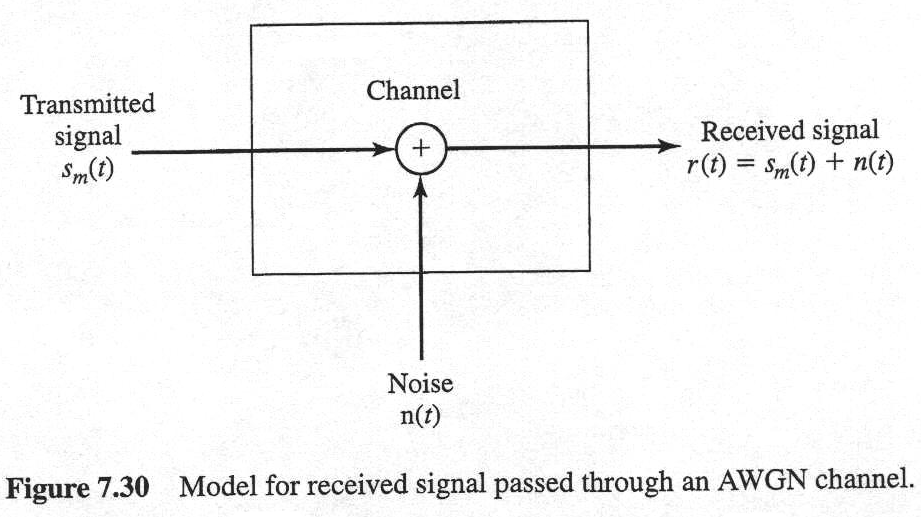
\includegraphics[scale = 0.5]{Ricevitore numerico.png}
\end{figure}

e lo schema del demodulatore (ricevitore) a correlatore (con le note): 

\begin{figure}[h]
    \centering
    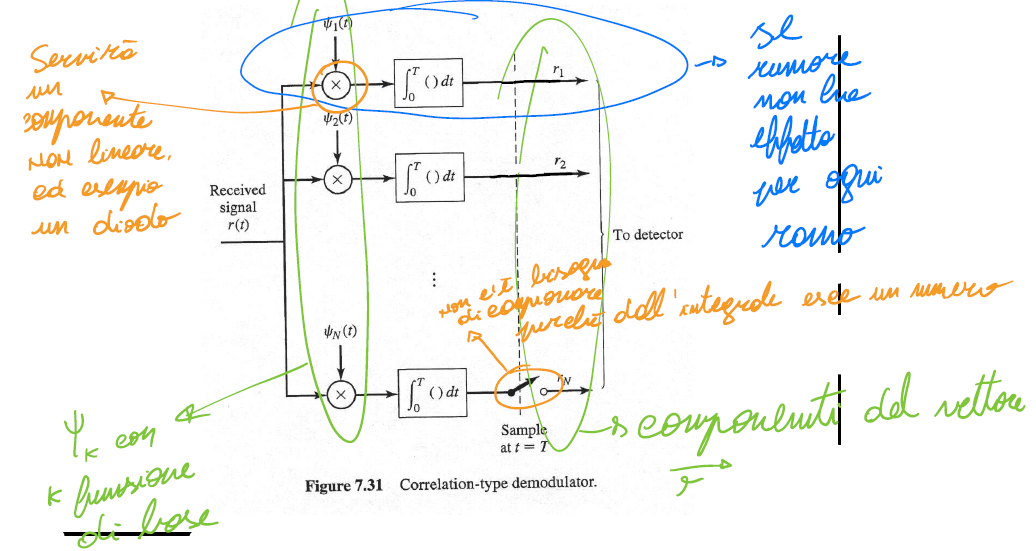
\includegraphics[scale = 0.5]{Demodulatore (ricevitore) a correlatore schema con note.PNG}
\end{figure} 

possiamo scrivere che la media nel singolo ramo del demodulatore a correlatore vale: 

{
    \Large 
    \begin{equation}
        \mathbb{E} [r_k] = \mathbb{E} [s_{mk} + n_k] = \mathbb{E} [s_{mk}] = s_{mk}
    \end{equation}
}

\begin{tcolorbox}
$\mathbb{E} [s_{mk}] = s_{mk}$ all'inizio sembra strano, ma guardati l'esempio della sezione successiva sull'esercizio della M-PAM. \newline 

Perché, per esteso dovrebbe essere $\mathbb{E} [s_{mk} (t)] = s_{mk}$, 
cioè la media nel tempo del segnale $s_{mk}$
\end{tcolorbox}

Inoltre poniamo che la varianza del rumore è uguale alla varianza del segnale, quindi: 

{
    \Large 
    \begin{equation}
        \sigma_r^{2} = \sigma_n^{2} = \frac{N_0}{2}
    \end{equation}
}

\begin{tcolorbox}
In questo caso, consideriamo il caso più semplice, cioè che il simbolo sia deterministico, e che quindi ha varianza nulla, 
ma su cui è sommato il rumore termico, che ha varianza $\frac{N_0}{2}$. \newline 

Quindi, la varianza totale da considerare del segnale ricevuto è uguale a quella del rumore termico
\end{tcolorbox}

Quindi, consideriamo la densità congiunta tra il vettore ricevuto e il vettore segnale trasmesso: 

{
    \Large 
    \begin{equation}
        f (\overrightarrow{r} | \overrightarrow{s_m})
        =
        \sum_{k = 1}^{N}
        f(r_k | s_{mk})
        \text{ per }
        m = 1, 2, \dots, M
    \end{equation}
}

Calcoliamo la densità condizionata perchè presupponiamo che sia stato trasmesso un determinato $\overrightarrow{s_m}$ (alche $\overrightarrow{s_m}$ lo consideriamo deterministico). \newline 

Considerano i singoli rami dal correlatore, possiamo scrivere: 

{
    \Large
    \begin{equation}
        f (r_k | s_{mk})
        = 
        \frac{1}{\sqrt{\pi \cdot N_0}}
        \cdot 
        \exp \left[- \frac{(r_k - s_{mk})^{2}}{N_0} \right]
        \text{ per }
        k = 1, 2, \dots, N
    \end{equation}
}

e quindi possiamo riscrivere la densità congiunta tra il vettore ricevuto e il vettore segnale trasmesso come: 


{
    \Large 
    \begin{equation}
        \begin{split}
        f (\overrightarrow{r} | \overrightarrow{s_m})
        &=
        \sum_{k = 1}^{N}
        f(r_k | s_{mk})
        \text{ per }
        m = 1, 2, \dots, M
        \\
        &\downarrow
        \\
        f (\overrightarrow{r} | \overrightarrow{s_m})
        &=
        \frac{1}{(\pi \cdot N_0)^{\frac{N}{2}}}
        \cdot 
        \exp \left[- \frac{\sum_{k=1}^{N}(r_k - s_{mk})^{2}}{N_0} \right] 
        \text{ per }
        m = 1, 2, \dots, M
        \\
        &=
         \frac{1}{(\pi \cdot N_0)^{\frac{N}{2}}}
        \cdot 
        \exp \left[- \frac{\abs{\overrightarrow{r} - \overrightarrow{s_m}}^{2}}{N_0} \right]
        \text{ per }
        m = 1, 2, \dots, M
    \end{split}        
    \end{equation}
}

dove con $\abs{\overrightarrow{r} - \overrightarrow{s_m}}$ si indica il modulo del vettore differenza che si ricava sottraendo 
il vettore $\overrightarrow{r}$ da $\overrightarrow{s_m}$. \newline 

\newpage 

\subsubsection{M-PAM con demodulatore a correlatore}
\footnote{Slide del prof | Ricevitore numerico | pag 5.1 \\  
Slide | Ricevitore numerico | pag 5.1 \\
Appunti | 2025-04-04 | pag 3
}

Ricordando che la M-PAM è formata da una sola funzione di base 
(vedi capitolo 7.3.0.1 Esempi di modulazioni con N = 1 pag 206), 
come ad esempio quella rettangolare: 

\begin{figure}[h]
    \centering
    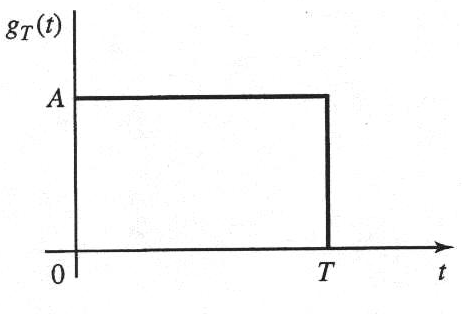
\includegraphics[scale = 1]{Funzione di base per una M-PAM.png}
\end{figure} 

Calcoliamo l'uscita del segnale dal demodulatore a correlatore : 

{
    \Large
    \begin{equation}
        \begin{split}
            r 
            &= 
            \int_{0}^{T}
            r(t) \cdot \Psi(t) dt 
            \\
            &=
            \int_{0}^{T}
            r(t) \cdot \frac{1}{\sqrt{T}} dt
            \\
            &=
            \frac{1}{\sqrt{T}}
            \cdot 
            \int_{0}^{T}
            r(t) dt
            \\
            &= 
            \frac{1}{\sqrt{T}}
            \cdot 
            \int_{0}^{T}
            \left[
                s_{m} (t) 
                + 
                n(t)
            \right]
            dt
            \\
            &=
            \frac{1}{\sqrt{T}}
            \cdot 
            \int_{0}^{T}
            s_{m} (t)
            dt 
            + 
            \frac{1}{\sqrt{T}}
            \cdot 
            \int_{0}^{T}
            n(t)
            dt
            \\ 
            &=  
            \frac{1}{\sqrt{T}}
            \cdot 
            \int_{0}^{T}
            s_{m} (t)
            dt 
            + 
            n
            \\
            &= 
            \frac{1}{\sqrt{T}}
            \cdot 
            \int_{0}^{T}
            s_{m} \cdot \Psi (t)
            dt 
            + 
            n
            \\
            &= 
            \frac{1}{\sqrt{T}}
            \cdot 
            \int_{0}^{T}
            s_{m} \cdot \frac{1}{\sqrt{T}}
            dt 
            + 
            n
            \\
             &= 
            \frac{1}{\sqrt{T}} 
            \cdot
            \frac{1}{\sqrt{T}}
            \cdot 
            s_{m}
            \int_{0}^{T} 
            dt 
            + 
            n
            \\
            &= 
            \frac{1}{T}
            \cdot 
            s_m
            \cdot 
            T
            + 
            n
            \\
            &= 
            s_m + n
        \end{split}
    \end{equation}
}

dove: 

{
    \Large 
    \begin{equation}
        s_m (t) = s_m \cdot \Psi (t)
    \end{equation}
}

e con n si indicano i contributi di rumore. \newline 

\begin{tcolorbox}
    Sembra un piccolo dettaglio, ma semplifica di tanto i calcoli
\end{tcolorbox} 

Quindi, utilizzando la formula precedente: 

{
    \Large 
    \begin{equation}
         f (\overrightarrow{r} | \overrightarrow{s_m})
        =
        \frac{1}{(\pi \cdot N_0)^{\frac{N}{2}}}
        \cdot 
        \exp \left[- \frac{\abs{\overrightarrow{r} - \overrightarrow{s_m}}^{2}}{N_0} \right]
    \end{equation}
}

e adattandola al caso N = 1 per la M-PAM, abbiamo che: 

{
    \Large 
    \begin{equation}
        f (r | s_m)
        = 
        \frac{1}{\sqrt{\pi \cdot N_0}}
        \cdot 
        \exp \left[ - \frac{(r - s_m)^{2}}{N_0}\right]
    \end{equation}
}

\newpage 

\section{Demodulatore (ricevitore) a filtri adattati (Matched-Filter)}
\footnote{Slide del prof | Ricevitore numerico | pag 5.2 - 6.1 \\  
Appunti di Damiano | pag 5.2 - 6.1\\
Slide | Ricevitore numerico | pag 5.2 - 6.1 \\
Appunti | 2025-04-04 | pag 4 \\ 
Appunti | 2025-07-21 Ricevimento | pag 6.2
}

Un altro tipo di demodulatore, oltre a quello a correlatore, 
è quello a filtri adattati (in inglese Matched-Filter). \newline 

Di seguito uno schema dell'architettura (con note): 

\begin{figure}[h]
    \centering
    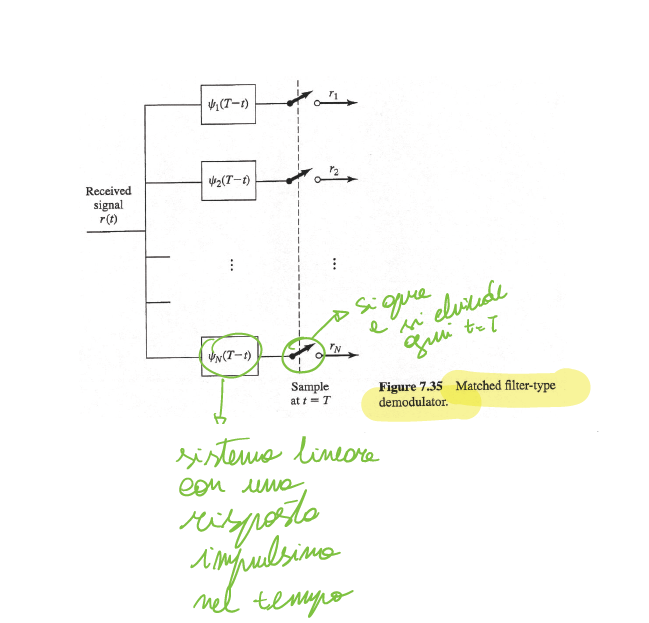
\includegraphics[scale = 1.2]{Demodulatore a filtri adattati.PNG}
\end{figure}

Rispetto al demodulatore a correlatore visto precedentemente: 

\begin{figure}[h]
    \centering
    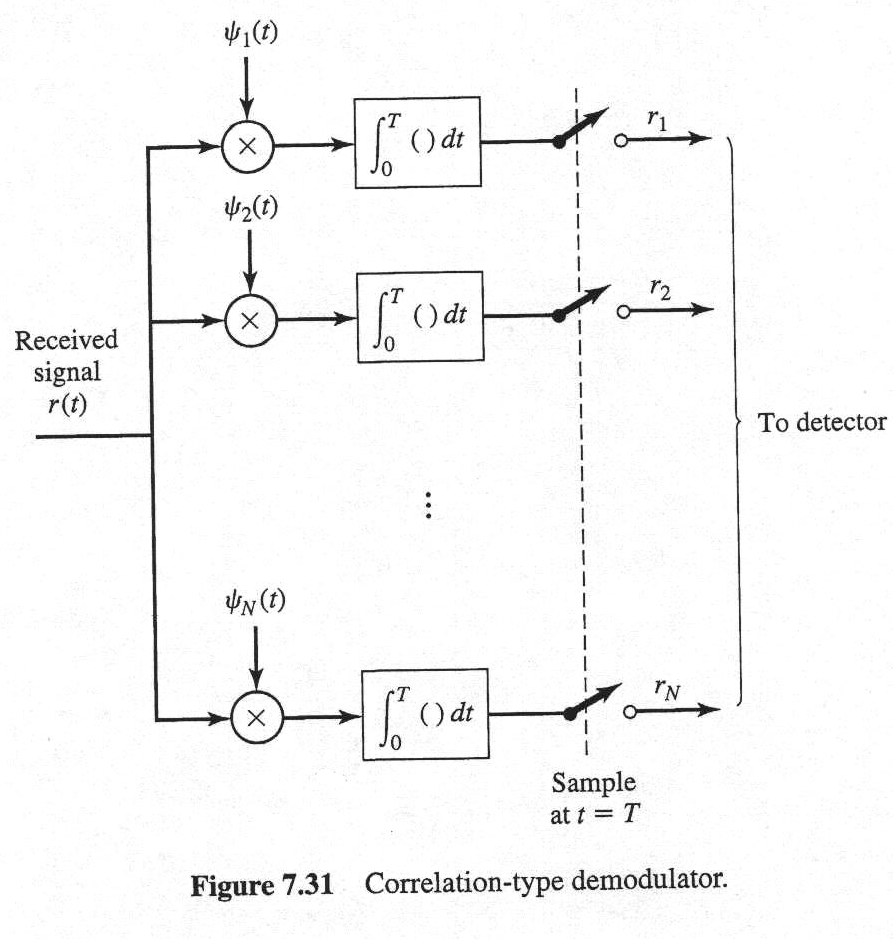
\includegraphics[scale = 0.3]{Demodulatore (ricevitore) a correlatore schema senza note.PNG}
\end{figure}

La formula che esce dal demodulatore a filtri adattati è la stessa del demodulatore a correlatore, 
ma, in questo caso, non ha bisogno di sistemi non lineari. \newline 

Come si vede dalla figura, non bisogna moltiplicare il singolo rame per la base (moltiplicare significa avere un componente non lineare come il diodo), 
bensì ci sono dei filtri, quindi sistemi e componenti lineari, 
con le rispettivi componenti della base. \newline 

Per quanto riguarda gli interruttori, qui vanno alzati e abbassati ogni tempo T. \newline 

La risposta impulsiva del sistema lineare nel singolo ramo k del demodulatore è il seguente: 

{
    \Large 
    \begin{equation}
        h_k (t) = \Psi_k (T - t) \text{ per } 0 \le t \le T
    \end{equation}
}

\begin{tcolorbox}
    Un breve ripasso da Tds: \\
    \url{https://github.com/ciccio25/appunti-teoria-dei-segnali/blob/main/Appunti%20Teoria%20dei%20segnali.pdf} \\
    Capitolo 5 - Sistemi lineari - pag 41
\end{tcolorbox}

Dal capitolo dei sistemi lineari, svolto nel precedente corso, 
sappiamo che l'uscita da un filtro $y_k (t)$ è la convoluzione tra il segnale di ingresso $r(\tau)$ e la risposta impulsiva del filtro $h_k (t)$. \newline 

In formule: 

{
    \Large 
    \begin{equation}
        y_k (t)
        = 
        \int_{- \infty}^{+ \infty}
        r(\tau) \cdot h_k (t-\tau) d\tau
    \end{equation}
}

Si vuole progettare un filtro che abbiamo, oltre l'intervallo che non ci serve: 

{
    \Large 
    \begin{equation}
        h_k (t) = 0 \text{ per } t < 0 \text{ e } t > T
    \end{equation}
}

quindi, riprendendo la formula impulsiva nel filtro in cui si fa una convoluzione, significa che: 

{
    \Large 
    \begin{equation}
        \begin{split}
            h_k (t -\tau) &= 0 \text{ per } t - \tau < 0 \text{ e } t - \tau > T
            \\
            &\downarrow
            \\
            h_k (t -\tau) &= 0 \text{ per } t  < \tau \text{ e } t - T  >  \tau
        \end{split}
    \end{equation}
}

oppure: 

{
    \Large 
    \begin{equation}
        h_k (t -\tau) = 0 \text{ per } \tau > t \text{ e }  \tau <  t - T  
    \end{equation}
}

Quindi possiamo limitare da $[-\infty, + \infty]$ all'intervallo $[t - T, t]$, 
e possiamo riscrivere l'equazione della convoluzione come: 

{
    \Large 
    \begin{equation}
        \begin{split}
        y_k (t)
        &= 
        \int_{- \infty}^{+ \infty}
        r(\tau) \cdot h_k (t-\tau) d\tau
       \\
       &\downarrow 
       \\ 
        y_k (t)
        &= 
        \int_{t - T}^{t}
        r(\tau) \cdot h_k (t-\tau) d\tau
    \end{split}
    \end{equation}
}

Siccome sappiamo che: 

{
    \Large 
    \begin{equation}
        h_k (t) = \Psi_k (T - t) \text{ per } 0 \le t \le T
    \end{equation}
}

possiamo cambiare ulteriormente la risposta impulsiva come: 

{
    \Large 
    \begin{equation}
        \begin{split}
            y_k (t)
        &= 
        \int_{t - T}^{t}
        r(\tau) \cdot h_k (t-\tau) d\tau
        \\
        &\downarrow
        \\ 
         y_k (t)
        &= 
        \int_{0}^{t}
        r(\tau) \cdot \Psi_k (T - t + \tau) d\tau
        \end{split}
    \end{equation}
}

dove k = 1 ,2 , $\dots$, N. \newline 

Ponendo: 

{
    \Large 
    \begin{equation}
        t = T
    \end{equation}
}

dove T è il periodo del segnale, allora possiamo considerare la risposta impulsiva nel periodo T del filtro: 

{
    \Large 
    \begin{equation}
        \begin{split}
           y_k (t)
        &= 
        \int_{0}^{t}
        r(\tau) \cdot \Psi_k (T - t + \tau) d\tau
        \\
        &\downarrow
        \\
        y_k (T)
        &= 
        \int_{0}^{T}
        r(\tau) \cdot \Psi_k (T - T + \tau) d\tau 
        \\
        &=
        \int_{0}^{T}
        r(\tau) \cdot \Psi_k (\tau) d\tau
        \\
        &= 
        r_k  
        \end{split}
    \end{equation}
}

dove: 

\begin{itemize}
    \item k = 1 ,2 , $\dots$, N 
    \item $r_k$ è un elemento del vettore $\overrightarrow{r}$ ricevuto 
\end{itemize}

\begin{tcolorbox}
    La scelta di utilizzare dei componenti lineari o non lineari in fase di progetto dipende da "quello che si ha a scaffale". \newline 

    Per la teoria, il prof preferisce utilizzare il demodulatore a filtri adattati perchè si fa una moltiplicazione in frequenza, 
    e che, grazie alla relazione tra tempo e frequenza studiata nel vecchio corso, implica una correlazione nel tempo. 

\end{tcolorbox} 


\newpage 

\subsection{Filtro adattato}
\footnote{Slide del prof | Ricevitore numerico | pag 6.2 - 7.1\\  
Appunti di Damiano | pag 6.2 - 7.1\\
Slide | Ricevitore numerico | pag 6.2 - 7.1 \\
Appunti | 2025-04-04 | pag 4
}

\begin{tcolorbox}
    Spiegazione di cosa è un filtro adattato in generale, 
    che non per forza deve essere collegato ad una trasmissione numerica.
\end{tcolorbox}

Un filtro la cui risposta impulsiva è: 

{
    \Large 
    \begin{equation}
        h(t) = s(T - t) \text{ per } 0 \le t \le T
    \end{equation}
}

si dice adattato al segnale s(t) (dove s(t) è il segnale di ingresso del filtro). \newline 

L'uscita del filtro vale: 

{
    \Large 
    \begin{equation}
        \begin{split}
            y(t)
            &= 
            \int_{0}^{t}
            s(\tau) \cdot h (t - \tau) d\tau
            \\
            &= 
            \int_{0}^{t}
            s(\tau) \cdot h (T - t + \tau) d\tau
        \end{split}
    \end{equation}
}

Consideriamo come esempio l'andamento nel tempo 
del segnale s(t) in ingresso al filtro adattato (figura a sinistra) 
e l'andamento del tempo della risposta impulsiva h(t) del filtro adattato: 

\begin{figure}[h]
    \centering
    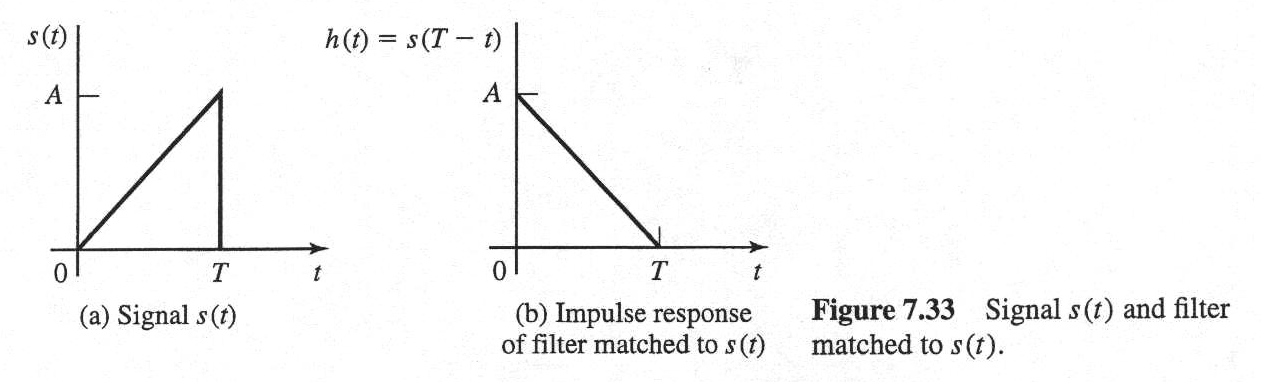
\includegraphics[scale = 0.7]{Esempio filtro adattato segnale ingresso e risposta impulsiva.png}
\end{figure}

L'uscita dal filtro adattato y(t) è la seguente: 

\begin{figure}[h]
    \centering
    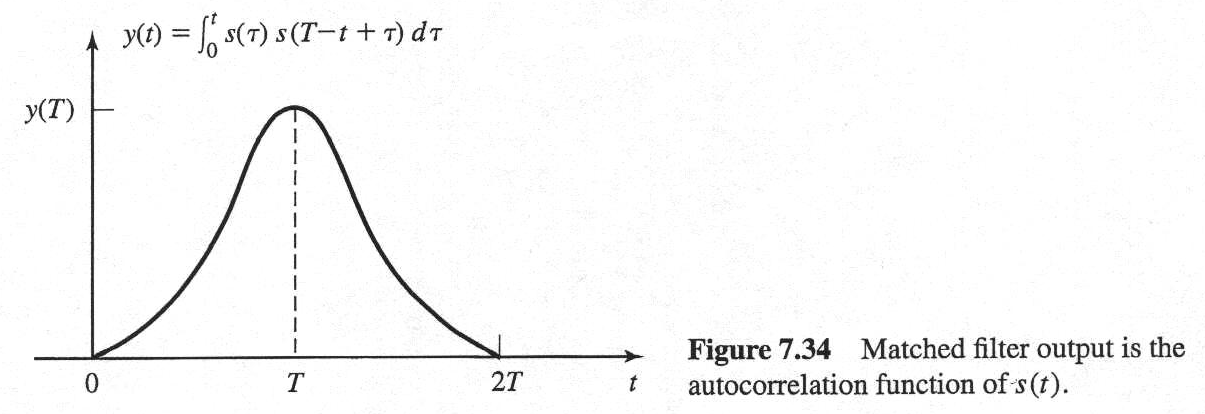
\includegraphics[scale = 0.7]{Esempio filtro adattato segnale in uscita.png}
\end{figure}

Generalmente si prende l'uscita y(t) al tempo t = T, perchè, come si nota dalla figura, si ha la potenza massima del filtro. \newline 

\newpage 

\subsubsection{Proprietà del filtro adattato}
\footnote{Slide del prof | Ricevitore numerico | pag 7.2 \\  
Appunti di Damiano | pag 7.2 \\
Slide | Ricevitore numerico | pag 7.2 \\
Appunti | 2025-04-04 | pag 4
}

Analizzando in frequenza, cioè in Fourier, la risposta impulsiva del filtro adattato: 

{
    \Large 
    \begin{equation}
        \begin{split}
            H (f)
            &=
            \int_{0}^{T}
            s(T - t) \cdot e^{- \jmath 2 \pi f t} dt
            \\
            &= 
            \left[ 
                \int_{0}^{T}
                s(\tau) \cdot e^{-\jmath 2 \pi f \tau} d\tau
            \right]
            \cdot 
            e^{-j 2 \pi f T} 
            \\
            &= 
            S^{*} (f) \cdot e^{-j 2 \pi f T} 
        \end{split}
    \end{equation}
}

Questi passaggi matematici dimostrano che la trasformata di Fourier di un filtro adattato h(t), cioè H(f), 
è uguale al complesso coniugato della trasformata di Fourier di s(t), cioè $S^{*}(f)$, 
ritardata di un tempo T: 
questo significa adattarsi al segnale di ingresso s(t). \newline 

Per quanto riguarda il modulo del filtro adattato: 

{
    \Large 
    \begin{equation}
        \abs{H (f)} = \abs{S(f)}
    \end{equation}
}

cioè il modulo del filtro adattato è uguale al modulo del segnale in ingresso. \newline 

\newpage 

\subsubsection{SNR in uscita dal filtro adattato}
\footnote{Slide del prof | Ricevitore numerico | pag 8.1 \\  
Appunti di Damiano | pag 8.1 \\
Slide | Ricevitore numerico | pag 8.1 \\
Appunti | 2025-04-04 | pag 5
}

\begin{tcolorbox}
    Ricordo che i calcoli matematici non ci servono al fine dell'esame orale. \newline 

    Servono solo per la dimostrazione. \newline 

    Le cose importanti sono le conclusioni e quello che scrivo a parole.
\end{tcolorbox}

Consideriamo l'uscita di un filtro adattato utilizzando la frequenza. \newline 

Avremo: 

{
    \Large 
    \begin{equation}
        \begin{split}
            y_s (t)
            &= 
            \int_{- \infty}^{+ \infty}
            Y(f) \cdot e^{\jmath 2 \pi f t} df 
            \\
            &=
            \int_{- \infty}^{+ \infty}
            \left[
                S(f) \cdot H(f)
            \right]
            \cdot e^{\jmath 2 \pi f t} df 
            \\
            &=
            \int_{- \infty}^{+ \infty}
                S(f) \cdot 
                \left[S^{*} (f) \cdot e^{- \jmath 2 \pi T} \right]
            \cdot e^{\jmath 2 \pi f t} df 
            \\
            &=
            \int_{- \infty}^{+ \infty}
                 \abs{S(f)}^{2} \cdot e^{- \jmath 2 \pi T} 
            \cdot e^{\jmath 2 \pi f t} df 
        \end{split}
    \end{equation}
}

Siccome consideriamo l'uscita al tempo t: 

{
    \Large
    \begin{equation}
        t = T
    \end{equation}
}

perchè abbiamo la potenza massima del filtro, allora l'uscita $y_s (t)$ diventa: 

{
    \Large 
    \begin{equation}
        \begin{split}
            y_s (t)
            &=
            \int_{- \infty}^{+ \infty}
                 \abs{S(f)}^{2} \cdot e^{- \jmath 2 \pi T} 
            \cdot e^{\jmath 2 \pi f t} df
            \\
            &\downarrow
            \\
            y_s (T)
            &=
            \int_{- \infty}^{+ \infty}
                 \abs{S(f)}^{2}  df
        \end{split}
    \end{equation}
} 

Grazie al teorema di Parseval: 

{
    \Large 
    \begin{equation}
        \abs{S(f)}^{2} = \abs{s(t)}^{2}
    \end{equation}
}

\begin{tcolorbox}
      Un breve ripasso da Tds: \\
    \url{https://github.com/ciccio25/appunti-teoria-dei-segnali/blob/main/Appunti%20Teoria%20dei%20segnali.pdf} \\
    Capitolo 4.2.1 - Teorema di Parseval - pag 32
\end{tcolorbox}

Quindi, possiamo scrivere: 

{
    \Large 
    \begin{equation}
        \begin{split}
            y_s (T)
            &=
            \int_{- \infty}^{+ \infty}
            \abs{S(f)}^{2}  df
            \\
            &\downarrow
            \\
            y_s (T)
            &=
            \int_{- \infty}^{+ \infty}
            \abs{s(t)}^{2}  df
            \\
            &= 
            E_s
        \end{split}
    \end{equation}
}

dove $E_s$ si intende l'energia del segnale. \newline 

Sapendo che la potenza del rumore $S_{n_0}$ è:

{
    \Large 
    \begin{equation}
       S_{n_0} (f) = \abs{H (f)}^{2} \cdot \frac{N_0}{2} 
    \end{equation}
}

La potenza del rumore $P_n$ vale: 

{
    \Large 
    \begin{equation}
        \begin{split}
            P_n 
            &= 
            \int_{- \infty}^{+ \infty}
            S_{n_0} (f) df
            \\
            &= 
            \int_{- \infty}^{+ \infty}
            \frac{N_0}{2} \cdot \abs{H(f)}^{2}
            df
            \\
            &= 
            \frac{N_0}{2} \cdot
            \int_{- \infty}^{+ \infty}
            \abs{H(f)}^{2}
            df
            \\
            &=
            \frac{N_0}{2} \cdot
            \int_{- \infty}^{+ \infty}
            \abs{S(f)}^{2}
            df 
            \\
            &= 
            \frac{N_0}{2} \cdot E_s
        \end{split}
    \end{equation}
}

Mettendo in relazione tutti i dati, calcoliamo il rapporto segnale rumore del filtro adattato: 

{
    \Large 
    \begin{equation}
        \begin{split}
            \left(
                \frac{S}{N}
            \right)_{o}
            &= 
            \frac{\left[y_s (T)\right]^{2}}{P_n}
            \\
            &= 
            \frac{(E_s)^{2}}{\frac{N_0}{2} \cdot E_s}
            \\
            &= 
            \frac{2 \cdot E_s}{N_0}
        \end{split}
    \end{equation}
}

Se ci mettiamo a t = T, 
con un filtro adattato, questo è il rapporto segnale rumore massimo in uscita. \newline 

\newpage 

\section{Decisore}
\footnote{Slide del prof | Ricevitore numerico | pag 8.2 - 9.1\\  
Appunti di Damiano | pag 8.2 - 9.1\\
Slide | Ricevitore numerico | pag 8.2 - 9.1 \\
Appunti | 2025-04-04 | pag 5 - 6 \\
Appunti | 2025-07-21 Ricevimento | pag 7
}

Come scritto precedentemente, 
in un ricevitore numerico, 
dopo il demodulatore è necessario un decisore. \newline 

Consideriamo come esempio grafico il caso di una trasmissione, dopo il demodulatore, 
in N = 3, con M = 4, nella costellazione: 

\begin{figure}[h]
    \centering
    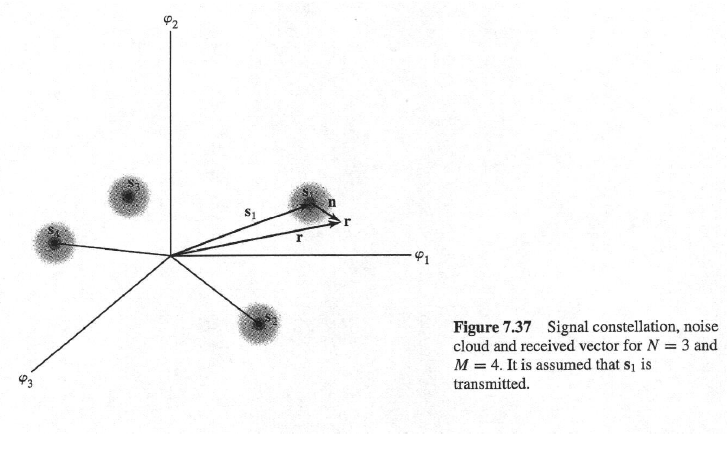
\includegraphics[scale = 1]{costellazione in N = 3 e M = 4 di esempio.PNG}
\end{figure}

Si considerano sistemi cooperanti. \newline 

\begin{tcolorbox}
Per sistemi cooperanti si intende che il decisore collabora con il demodulatore, 
cioè il demodulatore "passa" l'informazione del segnale ricevuto al decisore. \newline 

Se invece si considera un sistema non cooperante, il decisore dovrebbe prendere una decisione "alla cieca", 
da solo
\end{tcolorbox}

Spiegando graficamente la costellazione, 
se non consideriamo il rumore che riceviamo in trasmissione, 
in ricezioni dovremmo ricevere il vettore originariamente trasmesso. \newline 

Cioè, in formule, se non esistesse il rumore termico: 

{
    \Large 
    \begin{equation}
        \overrightarrow{r} = \overrightarrow{s_m}
    \end{equation}
}

MA, siccome esiste il rumore termico: 

{
    \Large 
    \begin{equation}
        \overrightarrow{r} \neq \overrightarrow{s_m}
    \end{equation}
}

Il rumore varia la posizione di $\overrightarrow{s_m}$ nella costellazione e, 
come indicato nella figura, $\overrightarrow{r}$ si troverà in un intorno di $\overrightarrow{s_m}$. \newline 

Inoltre, essendo il rumore termico AWGN un processo stocastico, quindi probabilistico, 
dobbiamo utilizzare la probabilità. \newline 

In questo caso, si possono calcolare due tipi di probabilità: 

\begin{itemize}
    \item probabilità massima, che è una probabilità che possiamo calcolare prima della trasmissione, cioè a priori 
    \item probabilità massima condizionata dal segnale ricevuto, che è una probabilità che possiamo solo dopo aver ricevuto il segnale $\overrightarrow{r}$, cioè a posteriori
\end{itemize}

Ovviamente, a noi interessa di più la seconda, quindi vogliamo calcolare la seguente probabilità: 

{
    \Large 
    \begin{equation}
        \Pr{\overrightarrow{s_m} | \overrightarrow{r}}
    \end{equation}
}
\newpage 

\subsection{Criterio MAP: Maximum A Posteriori probability}
\footnote{Slide del prof | Ricevitore numerico | pag 9.2 \\  
Appunti di Damiano | pag 9.2 \\ 
Slide | Ricevitore numerico | pag 9.2 \\
Appunti | 2025-04-04 | pag 6
}

Il decisore sarà comparativo: cioè confronterà la probabilità a priori di $\overrightarrow{s_m}$ e la confronterà con il segnale ricevuto $\overrightarrow{r}$. \newline 

In particolare, con il criterio MAP, 
il decisore seleziona, come segnale trasmesso, quello che massimizza la $\Pr {\overrightarrow{s_m} | \overrightarrow{r}}$: 

{
    \Large 
    \begin{equation}
        \Pr {\overrightarrow{s_m} | \overrightarrow{r}}
        = 
        \frac{f (\overrightarrow{r} | \overrightarrow{s_m}) \cdot \Pr {\overrightarrow{s_m}}}{f(\overrightarrow{r})}
    \end{equation}
}

\begin{tcolorbox}
    Questa formula è l'applicazione della formula di Bayes applicata alla costellazione, 
    quindi in ambito vettoriale. \newline 

    La avevamo già vista nel corso di Teoria dei Segnali. \newline 

    \url{https://github.com/ciccio25/appunti-teoria-dei-segnali/blob/main/Appunti%20Teoria%20dei%20segnali.pdf} \\
    Capitolo 12.5 - Eventi statisticamente indipendenti - pag 118 - 119 \newline 

    \begin{equation}
        \Pr{A | B} = \frac{\Pr{B | A} \cdot \Pr{A}}{\Pr{B}}
    \end{equation}
   

    Se invece sei un iPad kid (o iPad girl, qui non facciamo discriminazioni), 
    puoi vedere i seguenti video per capire meglio la formula di Bayes: 

    \begin{itemize}
        \item \url{https://www.youtube.com/watch?v=HZGCoVF3YvM&t=249s} \\ Bayes theorem, the geometry of changing beliefs by 3Blue1Brown (per visualizzare l'applicazione della formula di Bayes) 
        \item \url{https://www.youtube.com/watch?v=OByl4RJxnKA} \\ Bayes' Theorem of Probability With Tree Diagrams \& Venn Diagrams by The Organic Chemistry Tutor (per visualizzarla e fare dei semplici esercizi di calcolo)
    \end{itemize}

\end{tcolorbox}

Quindi per massimizzare la formula di $ \Pr {\overrightarrow{s_m} | \overrightarrow{r}}$, 
bisogna massimizzare il numeratore, 
quindi $f (\overrightarrow{r} | \overrightarrow{s_m}) \cdot \Pr {\overrightarrow{s_m}}$ deve essere la più grande possibile. \newline 

Calcolare $f (\overrightarrow{r} | \overrightarrow{s_m})$ significa confrontare il vettore $\overrightarrow{r}$ ricevuto con tutti i possibili $\overrightarrow{s_m}$ della costellazione. \newline 

Possiamo ignorare il denominatore perchè $f(\overrightarrow{r})$ è un fattore moltiplicativo, 
lo stesso vale per $\Pr {\overrightarrow{s_m}}$ . \newline 

Quindi alla fine, ciò che dovremmo massimizzare è $f (\overrightarrow{r} | \overrightarrow{s_m})$. \newline 

Inoltre, il criterio MAP è il miglior criterio di decisione a posteriori, 
ma lo si può applicare solo se i vettori $\overrightarrow{s_m}$ sono equiprobabili. \newline 

\newpage 

\subsection{Criterio ML: Maximum Likelihood}
\footnote{Slide del prof | Ricevitore numerico | pag 10.1 \\  
Appunti di Damiano | pag 10.1 \\
Slide | Ricevitore numerico | pag 10.1 \\
Appunti | 2025-04-04 | pag 6
}

Ipotizzando che i simboli dell'alfabeto sono equiprobabili, 
possiamo scrivere: 

{
    \Large 
    \begin{equation}
        \Pr{\overrightarrow{s_m}}
        = 
        \frac{1}{M}
    \end{equation}
}

Siccome dobbiamo massimizzare $f (\overrightarrow{r} | \overrightarrow{s_m})$, 
dalla sezione 8.2.2 Caratteristiche del vettore in uscita dal correlatore a pag 259, 
abbiamo visto che: 

{
    \Large 
    \begin{equation}
        f(\overrightarrow{r} | \overrightarrow{s_m})
        =
         \frac{1}{(\pi \cdot N_0)^{\frac{N}{2}}}
        \cdot 
        \exp \left[- \frac{\abs{\overrightarrow{r} - \overrightarrow{s_m}}^{2}}{N_0} \right]
        \text{ per }
        m = 1, 2, \dots, M
    \end{equation}
}

Siccome nella formula abbiamo un esponenziale, 
quindi con una semplice manipolazione matematica, 
possiamo scrivere: 

{
    \Large 
    \begin{equation}
        \begin{split}
               f(\overrightarrow{r} | \overrightarrow{s_m})
        &=
         \frac{1}{(\pi \cdot N_0)^{\frac{N}{2}}}
        \cdot 
        \exp \left[- \frac{\abs{\overrightarrow{r} - \overrightarrow{s_m}}^{2}}{N_0} \right]
        \\
        &\downarrow
        \\
        \ln 
        \left[
            f(\overrightarrow{r} | \overrightarrow{s_m})
        \right]
        &=
        - \frac{N}{2} 
        \cdot 
        \ln(\pi \cdot N_0)
        - 
        \frac{\abs{\overrightarrow{r} - \overrightarrow{s_m}}^{2}}{N_0}
        \\
        &=
        - \frac{N}{2} 
        \cdot 
        \ln(\pi \cdot N_0)
        - 
        \frac{D(\overrightarrow{r}, \overrightarrow{s_m})}{N_0} 
        \end{split}
    \end{equation}
}

dove con $D(\overrightarrow{r}, \overrightarrow{s_m})$ si intende la distanza 
tra i vettori $\overrightarrow{r}$ e $\overrightarrow{s_m}$. \newline 

Quindi, adesso dobbiamo calcolare la minima distanza 
$D(\overrightarrow{r}, \overrightarrow{s_m})$ perchè tutti gli altri parametri sono costanti. \newline 

\newpage 

\subsection{Distanza Euclidea minima}
\footnote{Slide del prof | Ricevitore numerico | pag 10.2 \\  
Appunti di Damiano | pag 10.2 \\ 
Appunti | 2025-07-21 Ricevimento | pag 8.1
}

Esplodendo la formula di $D(\overrightarrow{r}, \overrightarrow{s_m})$ nei vari componenti della base N del vettore, 
possiamo sviluppare il quadrato come: 

{
    \Large 
    \begin{equation}
        \begin{split}
            D(\overrightarrow{r}, \overrightarrow{s_m}) 
            &= 
            \abs{\overrightarrow{r} - \overrightarrow{s_m}}^{2}
            \\
            &= 
            \abs{\overrightarrow{r}}^{2}
            - 2 \cdot \overrightarrow{r} \cdot \overrightarrow{s_m}
            + 
            \abs{\overrightarrow{s_m}}^{2}
        \end{split} 
    \end{equation}
}
per m = 1, 2, $\dots$, M. \newline 

Quindi per minimizzare la distanza $ D(\overrightarrow{r}, \overrightarrow{s_m}) $, 
dobbiamo minimizzare i termini $- 2 \cdot \overrightarrow{r} \cdot \overrightarrow{s_m} + \abs{\overrightarrow{s_m}}^{2}$. \newline 

Il decisore individua il vettore $\overrightarrow{s_m}$ che minimizza: 

{
    \Large 
    \begin{equation}
        D^{'} (\overrightarrow{r}, \overrightarrow{s_m}) 
        = 
        - 2 \cdot \overrightarrow{r} \cdot \overrightarrow{s_m} + \abs{\overrightarrow{s_m}}^{2}
    \end{equation}
}

cioè applicando la metrica di distanza. \newline 

Oppure equivalentemente, il vettore $\overrightarrow{s_m}$ che massimizza: 

{
    \Large 
    \begin{equation}
        C(\overrightarrow{r}, \overrightarrow{s_m})
        = 
        2 \cdot \overrightarrow{r} \cdot \overrightarrow{s_m} - \abs{\overrightarrow{s_m}}^{2}
    \end{equation}
}

cioè applicando la metrica di correlazione. \newline 

Per i formati in cui i simboli hanno tutti la stessa energia, 
nel calcolo di $D^{'} (\overrightarrow{r}, \overrightarrow{s_m}) $ o di $C(\overrightarrow{r}, \overrightarrow{s_m})$, 
il termine $\abs{\overrightarrow{s_m}}^{2}$ può essere ignorato. \newline 

\begin{tcolorbox}
La distanza minima $D^{'} (\overrightarrow{r}, \overrightarrow{s_m}) $ è l'opposto della correlazione  $C(\overrightarrow{r}, \overrightarrow{s_m})$. \newline 

Quindi bisogna avere sia $\overrightarrow{r}$ e $\overrightarrow{s_m}$ per calcolare questi due parametri: 
ciò è possibile solo in sistemi cooperanti
\end{tcolorbox}

\iffalse
\newpage 

\subsubsection{MAP sulla 2-PAM}
\footnote{Slide del prof | Ricevitore numerico | pag 10.2 \\  
Appunti di Damiano | pag 10.2 
}

\begin{tcolorbox}
    Di seguito un esempio della MAP sulla 2-PAM. \newline 

    Sono formule, quindi puoi ignorarle.
\end{tcolorbox}

\begin{tcolorbox}[colback=green!5!white,colframe=green!75!black]
    TO-DO: FARE DA PAG 11 A PAG 19 DEL PDF E RICOPIARLE QUI
\end{tcolorbox}
\fi 

\newpage 

